The following cross checks were requested during approval:
\begin{itemize}
\item Take the Z+jets MC sample and define the scale factor based on the
overall number of events after the preselection in the signal dijet mass
window with respect to the sideband mass windows. Apply this constant scale
factor to the differential distribution of 4-body mass in the Z+jets events
in the sideband and see if you reproduce that for the signal region in the
entire mass range.

\item Compare the 4-body mass distributions for the lower and upper sideband in
the data and see if the ratio is constant with the 4-body mass.

\item Make a technical check of the last steps of the analysis, just to be safe.

\item Make the combination with 7 TeV as published (this was a condition at the pre-approval in fact).

\item Consider stopping the analysis at 600 GeV in light of the concerns.

\end{itemize}

\subsection{}

As can be seen in Figure~\ref{fig:clos} the tail is basically the same, implying that there is no issue
in the shape due to jet merging or so. In the low mass region there is a clear
difference, but this has already been studied in the past and it is due to the
bias from the mJJ selection.

However, this is not a closure test as one may think on such: if it is intended to
validate our analysis methodology, it is not the proper test, since this is not
what we do in the analysis (more below). If it is to check that the shapes are
the same, they are not... and we know that: the mllJJ and mJJ variables are not
fully decoupled (specially at low masses) and therefore there are differences.

It should be added that in our analysis we are not taking the shape of the SB
for anything except to validate the MC expectations. The shape in the SB does
not have any influence in the result. It has been relevant of course in the
decision to unblind the analysis, but only that. We are not using it in any way
to infer the shape in the SR for Z+jets (that is what the test above seems to
suggest).
Only the normalization in the SB has some impact on the result.

In our analysis, we are not assuming that the shape from the SB is able to
reproduce the SR. Even if at high masses they agree (because the requirement on
mJJ has smaller influence), we are not using that information.
We are extracting the expected shape from the same SR but the MC and we are
assuming that MC reproduces the SR as well as the SB. In fact today we know that
the MC reproduces the shape in BOTH SB, so assuming it also works in the SR is
the natural thing to do. We have no reason to think that there is something in
the Z-peak region affecting Z+jets that does not affect any of the two SB, one
at lower masses and the other at higher masses.

Furthermore (last but not least), we did not claim that the shape in the MC is
perfectly reproduced and we have a systematic uncertainty. As shown in the
approval talk, we quote a large systematic on the shape that covers by far any
discrepancy observed in the SB regions (plots this morning).
Recall the systematic is really large at high masses.

\begin{figure}[htb]
\centerline{
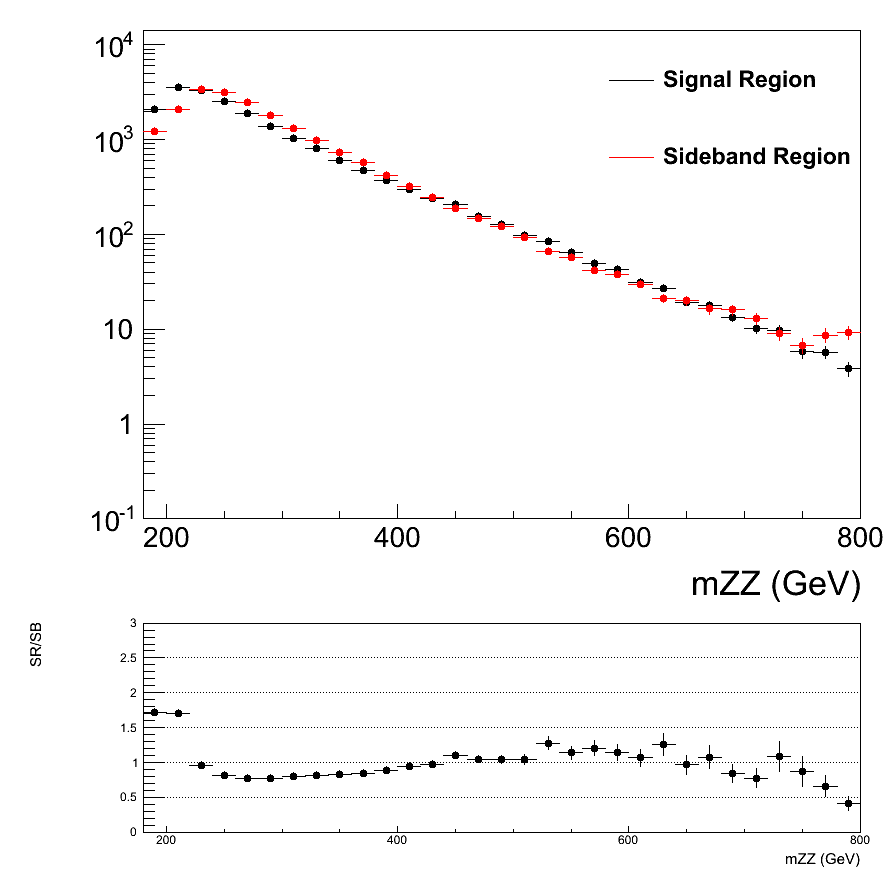
\includegraphics[width=0.33\textwidth]{plots/approvalxchecks/mZZ_SRvsSB_lep0_0btags_Log.png}
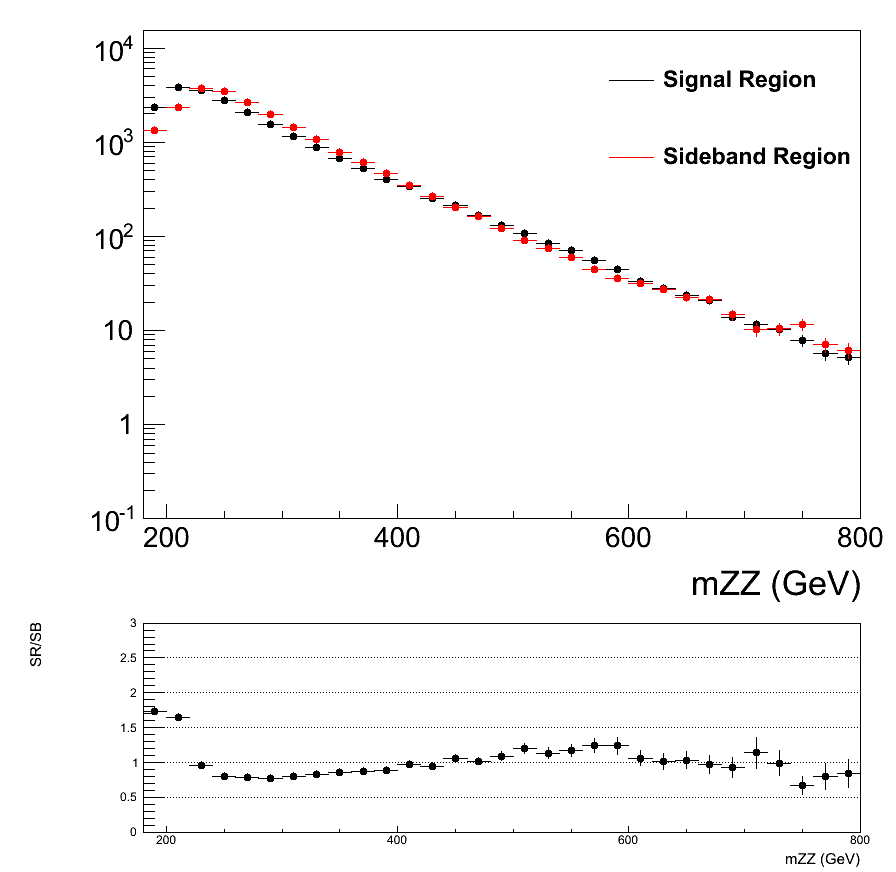
\includegraphics[width=0.33\textwidth]{plots/approvalxchecks/mZZ_SRvsSB_lep1_0btags_Log.png}
}
\centerline{
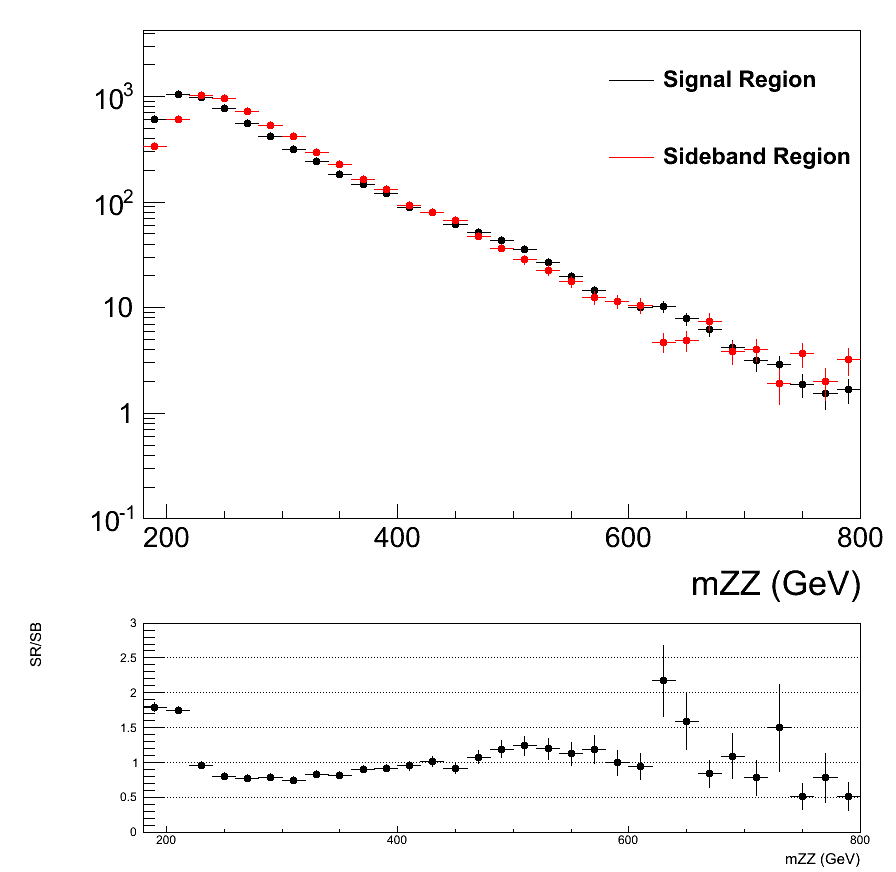
\includegraphics[width=0.33\textwidth]{plots/approvalxchecks/mZZ_SRvsSB_lep0_1btags_Log.png}
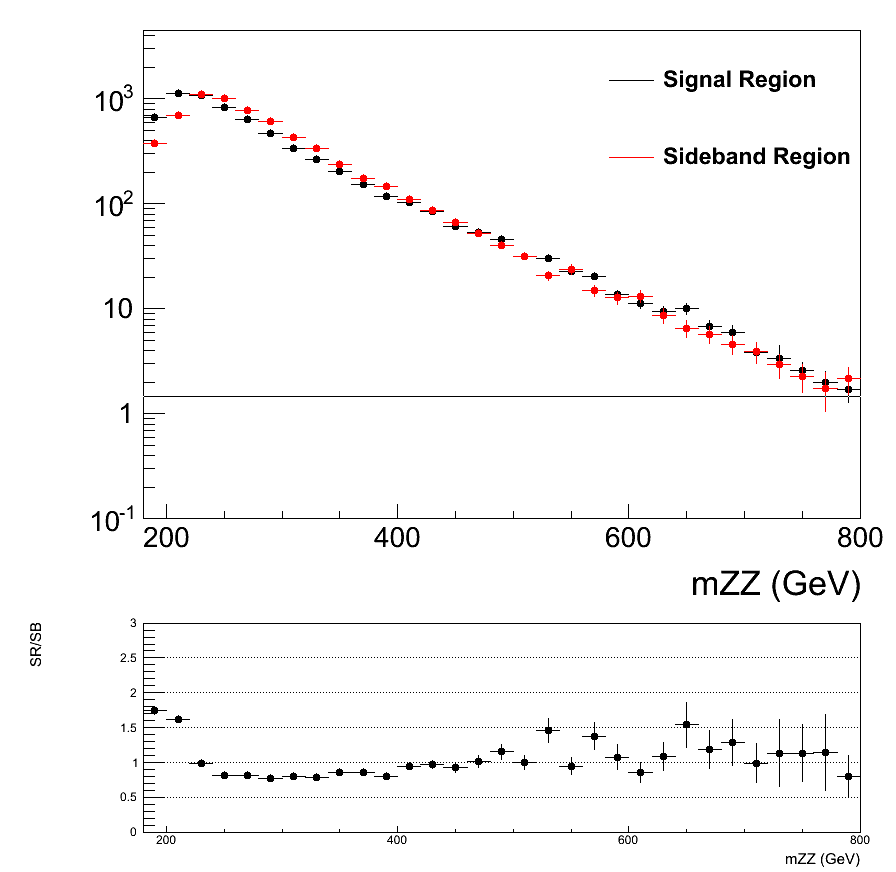
\includegraphics[width=0.33\textwidth]{plots/approvalxchecks/mZZ_SRvsSB_lep1_1btags_Log.png}
}
\centerline{
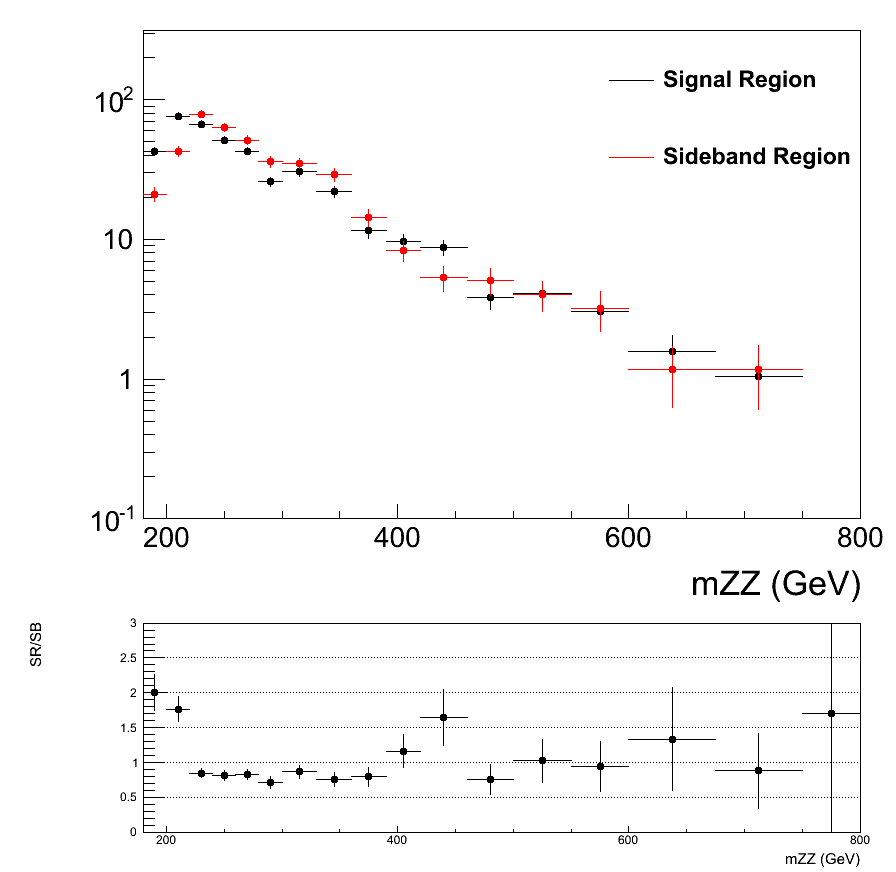
\includegraphics[width=0.33\textwidth]{plots/approvalxchecks/mZZ_SRvsSB_lep0_2btags_Log.png}
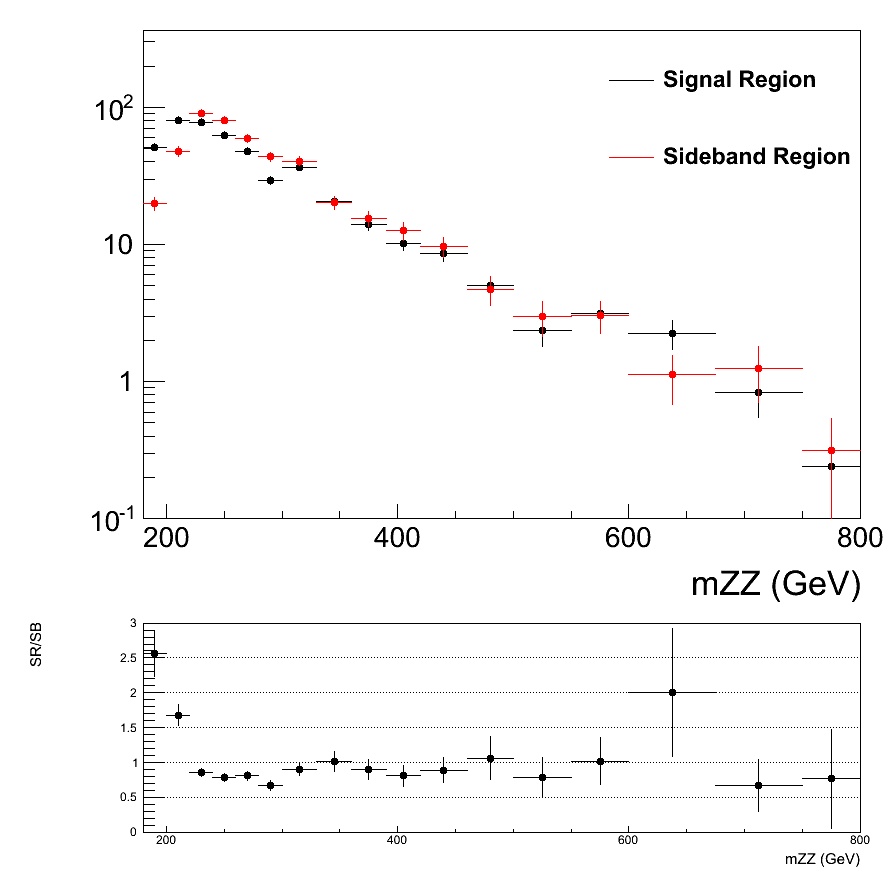
\includegraphics[width=0.33\textwidth]{plots/approvalxchecks/mZZ_SRvsSB_lep1_2btags_Log.png}
}
\caption{Mass distributions of the $\LL jj$ system for events in the simualted sideband and signal regions for the elctron (left)
 and muon (right) channels. From top to bottom, plots
correspond to the 0-, 1-, and 2-btag categories. 
\label{fig:clos}
}
\end{figure}


\subsection{}
Figure~\ref{fig:lrline} to~\ref{fig:lrlogmu} show the sideband data compared to the background prediction separately for the left and right sideband. While the background shapes are noticeably different between the left and right sideband, both agree well between data nad simulation, giving conifdence that the description is similarly good in the signal region. 


\begin{figure}[htb]
\centerline{
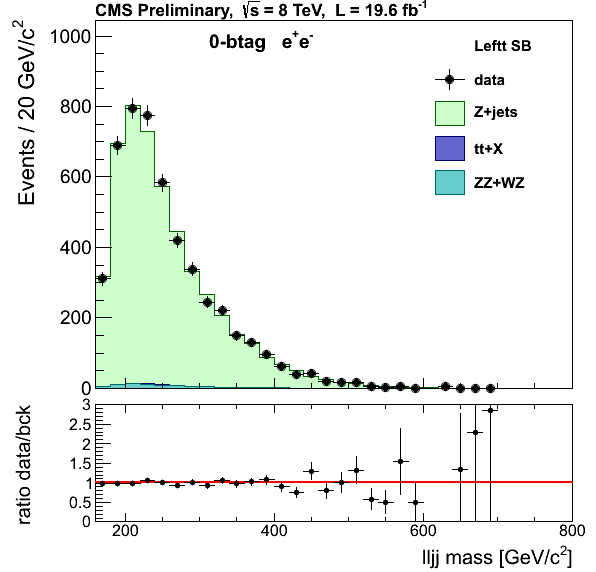
\includegraphics[width=0.33\textwidth]{plots/approvalxchecks/Left_0b_eelin.png}
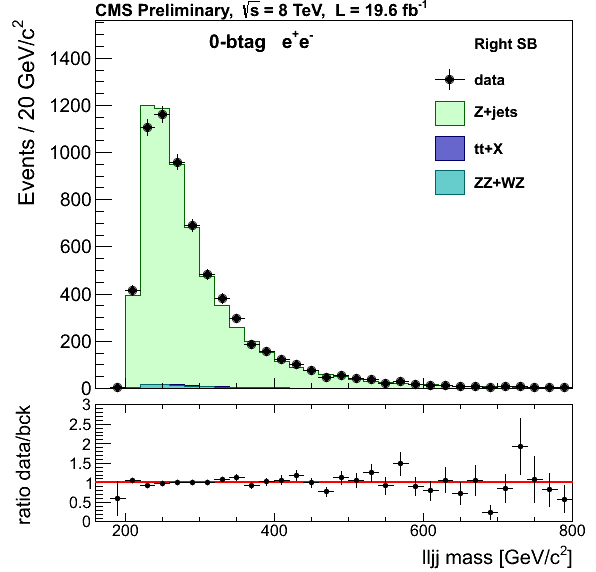
\includegraphics[width=0.33\textwidth]{plots/approvalxchecks/Right_0b_eelin.png}
}
\centerline{
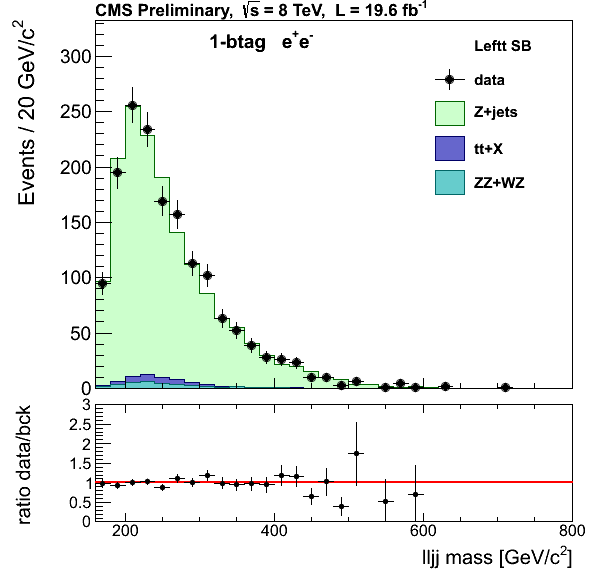
\includegraphics[width=0.33\textwidth]{plots/approvalxchecks/Left_1b_eelin.png}
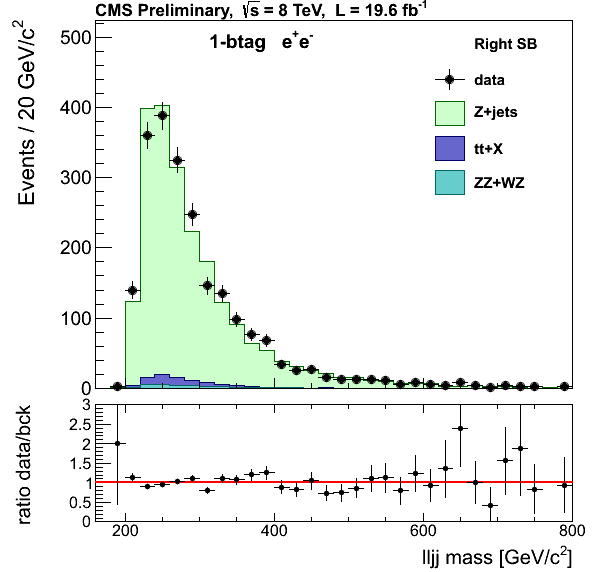
\includegraphics[width=0.33\textwidth]{plots/approvalxchecks/Right_1b_eelin.png}
}
\centerline{
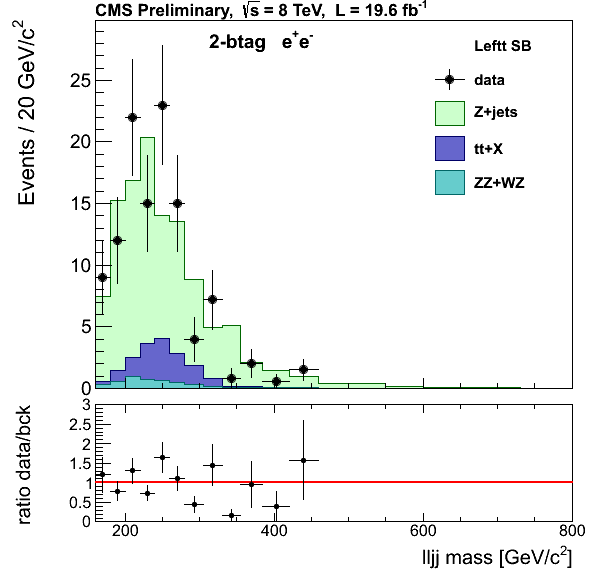
\includegraphics[width=0.33\textwidth]{plots/approvalxchecks/Left_2b_eelin.png}
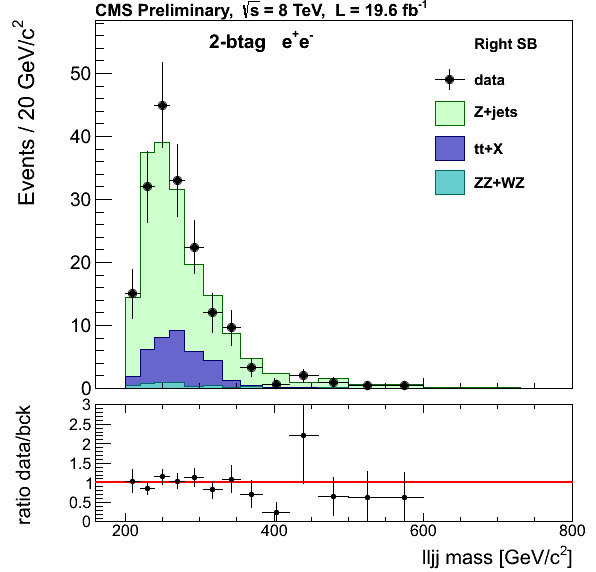
\includegraphics[width=0.33\textwidth]{plots/approvalxchecks/Right_2b_eelin.png}
}
\caption{Mass distributions of the $\LL jj$ system for events in the left (left)
 and right (right) sideband regions in the electron channel. From top to bottom, plots
correspond to the 0-, 1-, and 2-btag categories. 
The dots are data, pale green histogram corrected Z+jets simulation,
light blue simulated diboson background and dark blue $\ttbar$ events from data (which
include single top, WW, $\Zo\to\TT$+jets).
\label{fig:lrline}
}
\end{figure}

\begin{figure}[htb]
\centerline{
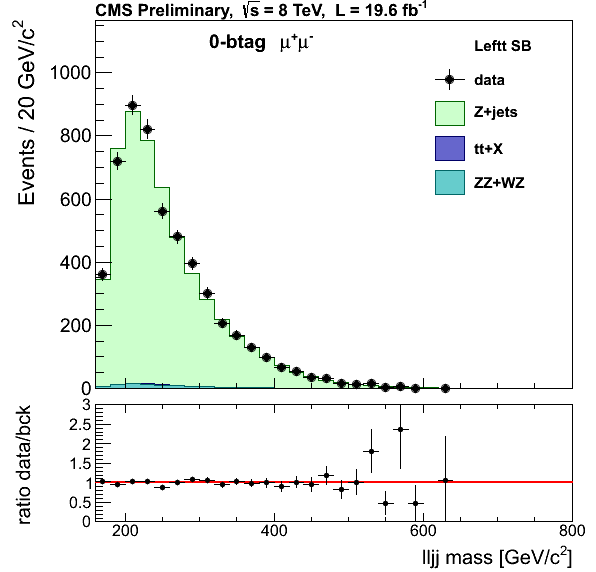
\includegraphics[width=0.33\textwidth]{plots/approvalxchecks/Left_0b_mmlin.png}
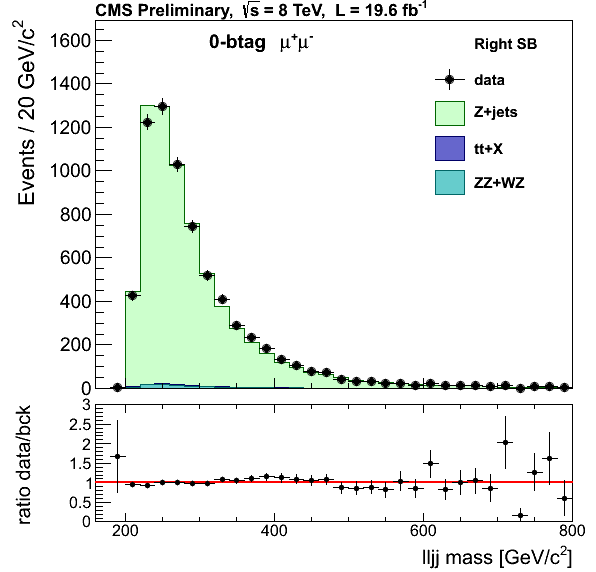
\includegraphics[width=0.33\textwidth]{plots/approvalxchecks/Right_0b_mmlin.png}
}
\centerline{
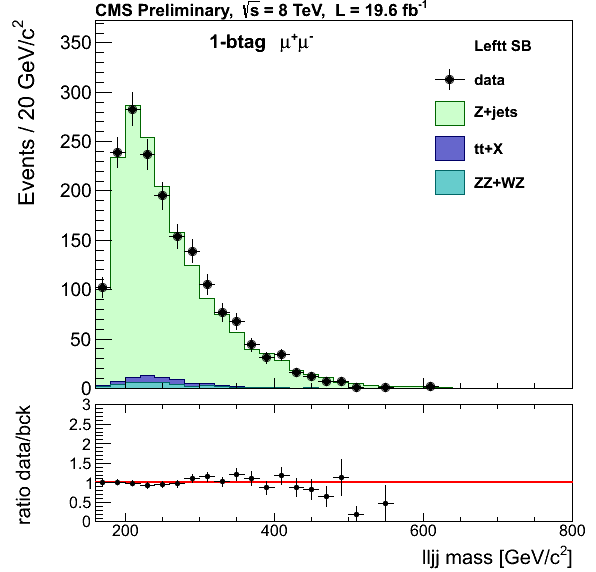
\includegraphics[width=0.33\textwidth]{plots/approvalxchecks/Left_1b_mmlin.png}
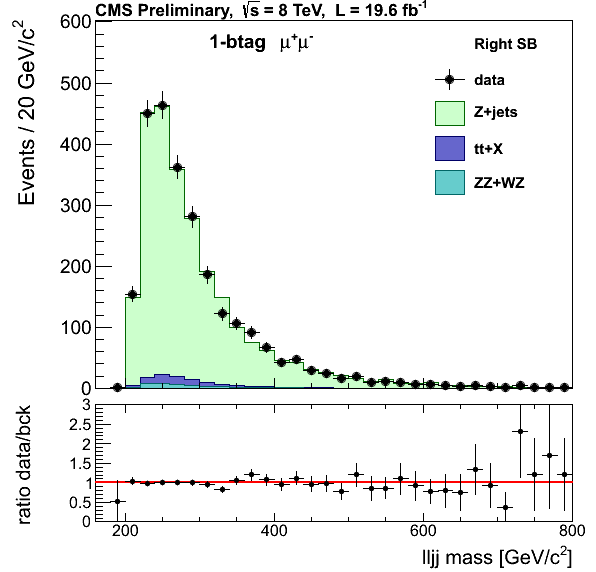
\includegraphics[width=0.33\textwidth]{plots/approvalxchecks/Right_1b_mmlin.png}
}
\centerline{
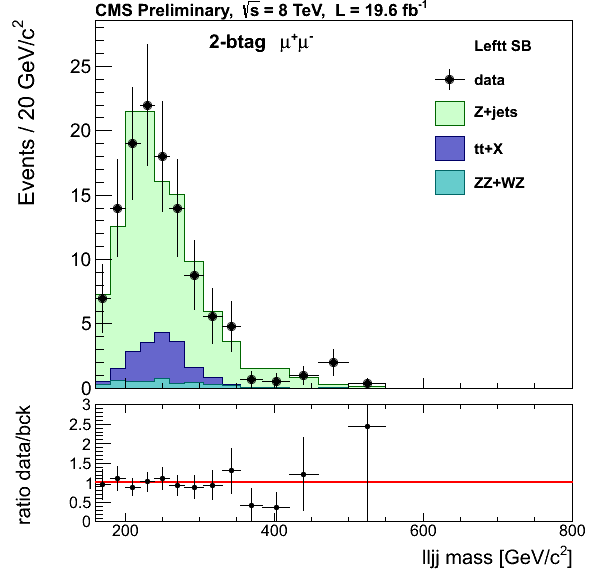
\includegraphics[width=0.33\textwidth]{plots/approvalxchecks/Left_2b_mmlin.png}
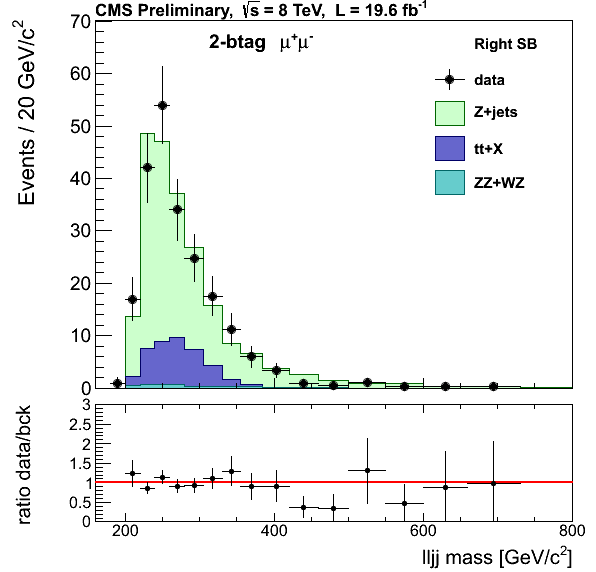
\includegraphics[width=0.33\textwidth]{plots/approvalxchecks/Right_2b_mmlin.png}
}
\caption{Same Figure~\ref{fig:lrline} but in themuon channel.
\label{fig:lrlinmu}
}
\end{figure}

\begin{figure}[htb]
\centerline{
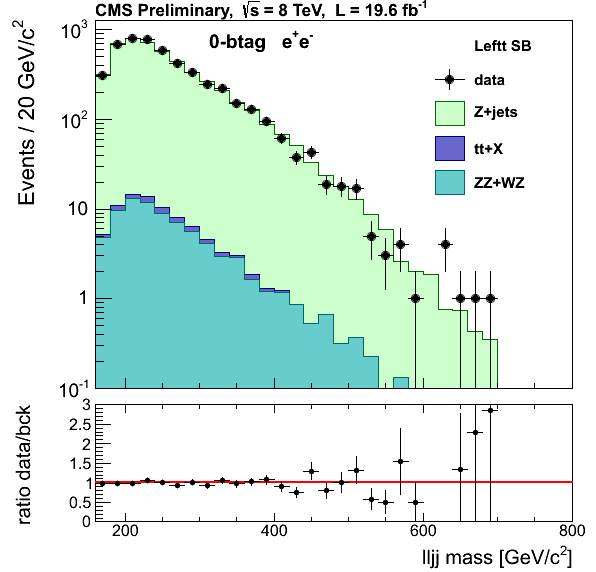
\includegraphics[width=0.33\textwidth]{plots/approvalxchecks/Left_0b_ee.png}
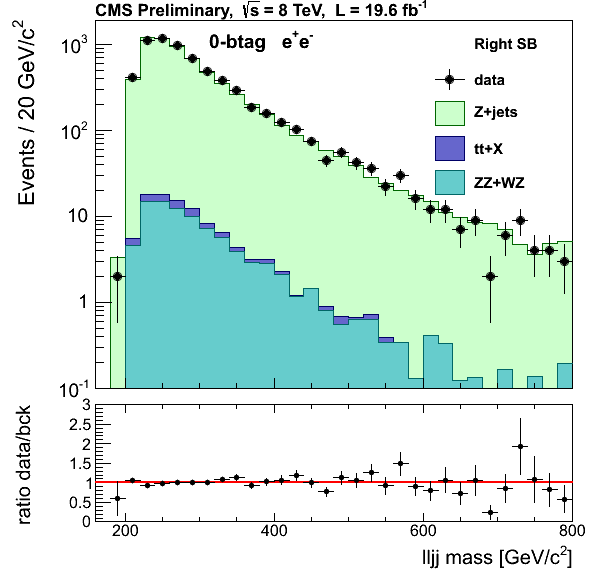
\includegraphics[width=0.33\textwidth]{plots/approvalxchecks/Right_0b_ee.png}
}
\centerline{
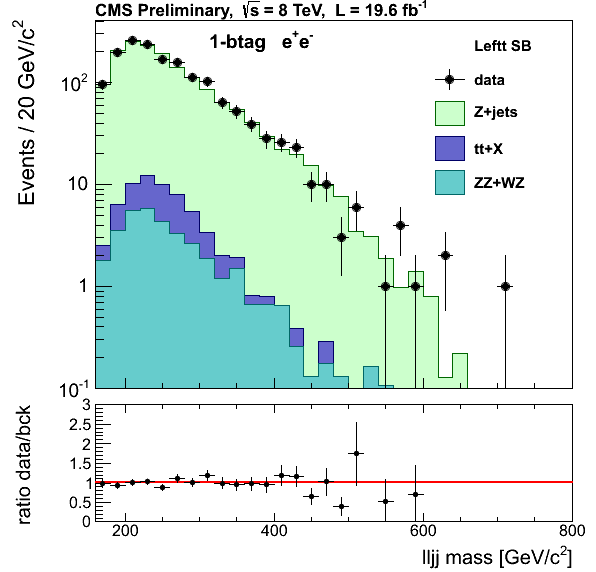
\includegraphics[width=0.33\textwidth]{plots/approvalxchecks/Left_1b_ee.png}
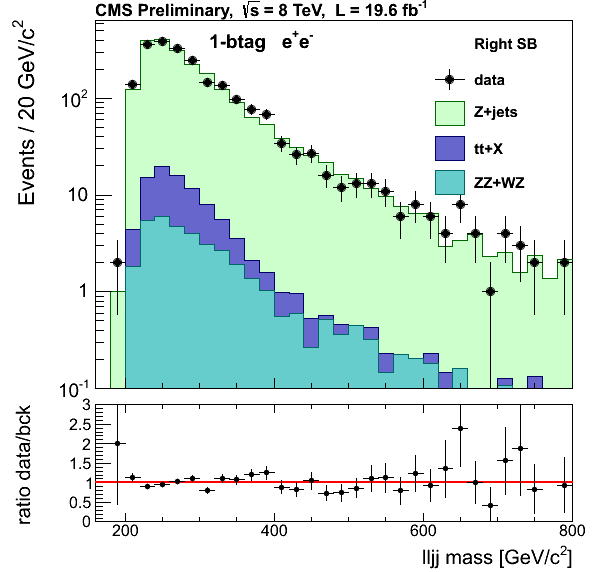
\includegraphics[width=0.33\textwidth]{plots/approvalxchecks/Right_1b_ee.png}
}
\centerline{
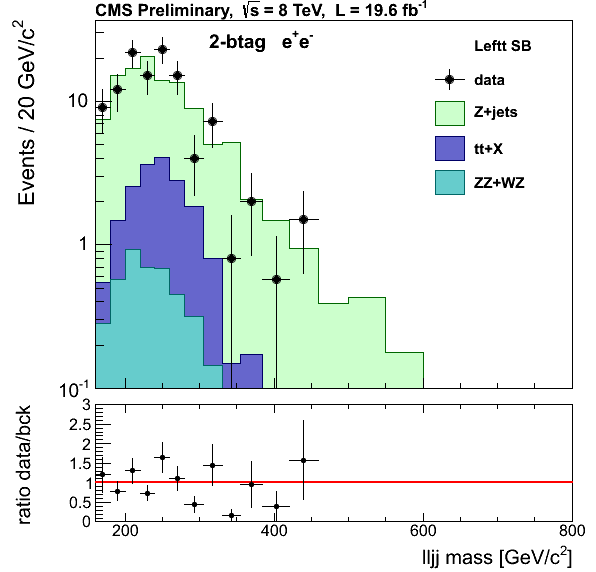
\includegraphics[width=0.33\textwidth]{plots/approvalxchecks/Left_2b_ee.png}
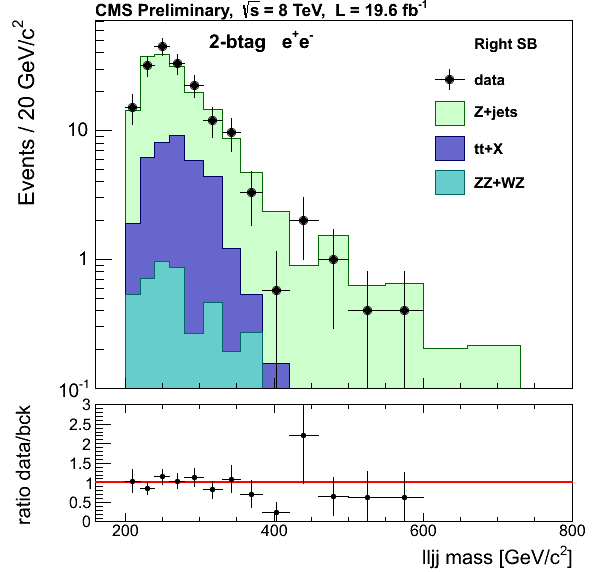
\includegraphics[width=0.33\textwidth]{plots/approvalxchecks/Right_2b_ee.png}
}
\caption{Same Figure~\ref{fig:lrline} but in themuon channellogarithmic scale.
\label{fig:lrloge}
}
\end{figure}

\begin{figure}[htb]
\centerline{
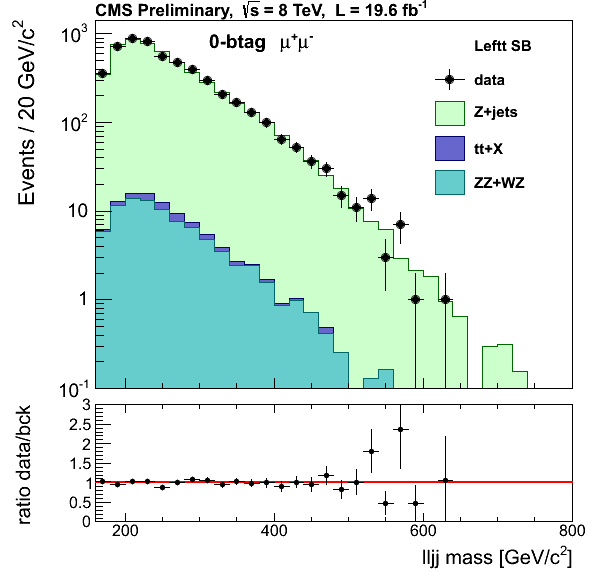
\includegraphics[width=0.33\textwidth]{plots/approvalxchecks/Left_0b_mm.png}
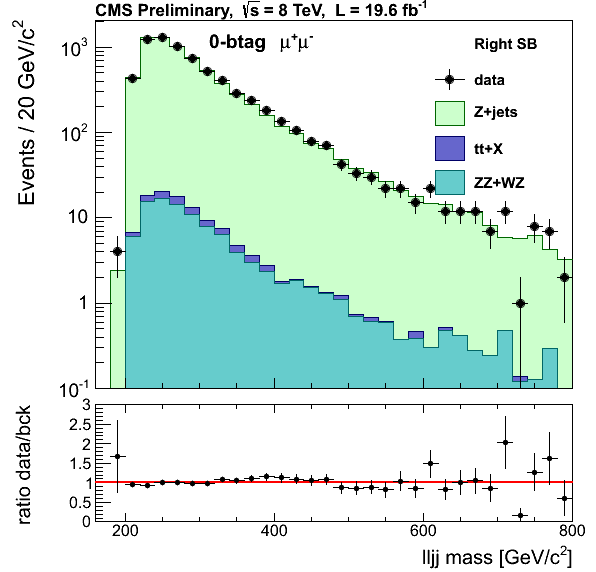
\includegraphics[width=0.33\textwidth]{plots/approvalxchecks/Right_0b_mm.png}
}
\centerline{
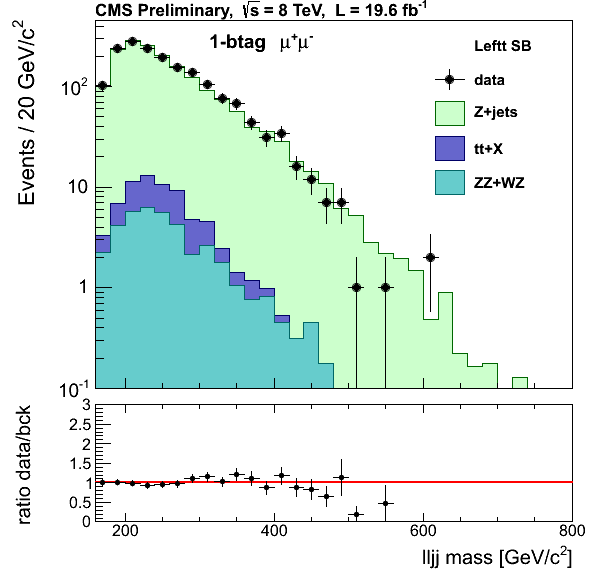
\includegraphics[width=0.33\textwidth]{plots/approvalxchecks/Left_1b_mm.png}
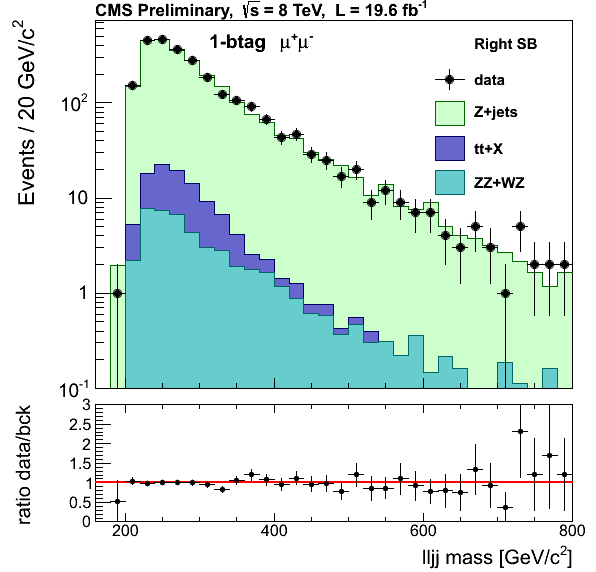
\includegraphics[width=0.33\textwidth]{plots/approvalxchecks/Right_1b_mm.png}
}
\centerline{
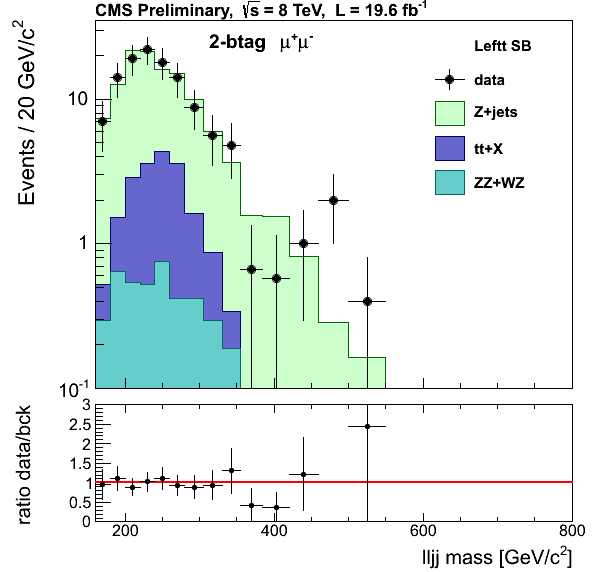
\includegraphics[width=0.33\textwidth]{plots/approvalxchecks/Left_2b_mm.png}
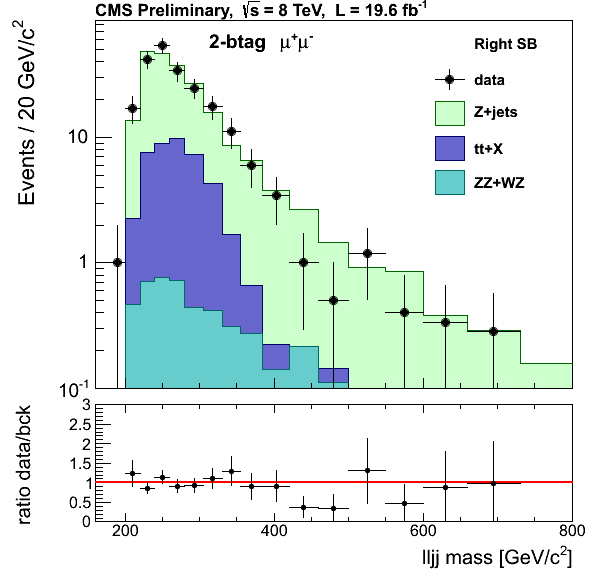
\includegraphics[width=0.33\textwidth]{plots/approvalxchecks/Right_2b_mm.png}
}
\caption{Same Figure~\ref{fig:lrlinmu} but in themuon channellogarithmic scale.
\label{fig:lrlogmu}
}
\end{figure}


\subsection{}
We have three independent analyses (different codes, ntuples, etc.) which agree 
well at the sub-percent level, in the numbers of events and shapes of the 
distributions. We have also checked the final limits, calculated both with the 
official combine tool and with an independent home-made code, and give 
consistent results. These checks have been reported in HZZ meetings and at the 
pre-approval session.

We are confident that no bug is present that gives visible effects.

\subsection{}
see section~\ref{sec:results}

\subsection{}
This has been addressed in the PAS. For internal documentation we keep the wider range in this note.


